\documentclass[11pt, spanish]{article}

\usepackage[spanish]{babel}
\selectlanguage{spanish}
\usepackage[utf8]{inputenc}
\usepackage{graphicx}
\usepackage{fancyhdr}
\usepackage{amsmath, amssymb}
\usepackage{enumerate}

\graphicspath{ {./img/} }


\pagestyle{fancy}
\fancyhf{}
\rhead{201111578 \\ 201317343}
\lhead{Sebastián Valencia Calderón \\ Edgar Daniel Gómez}
\rfoot{\thepage}

\begin{document}

\section{VA Discretas y Continuas de Mayor Aplicación}

\begin{enumerate}[(a)]

\item Según estándares FIFA, un balón oficial debe de tener una presión de aire entre
8.5 y 15.6 psi. Si la empresa Tygol establece que una válvula es defectuosa si no logra
mantener dicho estándar de presión, calcule la probabilidad de que una válvula fabricada por
el proveedor sea defectuosa.

\item ¿Cuál es la probabilidad de que se decida iniciar la producción de los nuevos
balones en la Etapa 1, sin pasar a la Etapa 2?

\item ¿Cuál es la probabilidad de que se deba posponer la producción en la Etapa 1, sin
pasar a la Etapa 2?

\item Si luego de la primera etapa se sabe que es necesario realizar la Etapa 2 de
control de calidad, ¿cuál es la probabilidad de que se acepte la producción bajo los criterios de
esta etapa?

\item El gerente del área de control de calidad ha decidido recolectar una muestra
aleatoria de 5 balones que presenten fallas en las válvulas, para inspeccionar los aspectos
específicos que ocasionan las fallas. Si el gerente inspecciona uno a uno los balones que
salen de la línea de producción, ¿cuál es la probabilidad de que deban inspeccionar 80
balones hasta completar la muestra requerida?

\item Calcule la probabilidad de que el décimo y el onceavo balón que inspecciona el
gerente sean los dos primeros balones que presenten fallas.

\item Bajo el contexto del literal $e)$ ¿cuál es el número esperado de balones que no
presentan fallas en las válvulas, que el gerente esperaría encontrar antes de completar su
muestra de 5 balones defectuosos?

\item Se envían 100 balones al proveedor de válvulas para que realice otras pruebas
relacionadas al desgaste de las mismas. Se sabe de antemano que entre los balones
enviados hay 30 que presentan fallas. Calcule la probabilidad de que, si el proveedor toma
una muestra aleatoria de 20 de estos 100 balones, encuentre a lo sumo 6 que presenten
fallas.

\end{enumerate}

\pagebreak
\section{Proceso de Poisson y Distribución Exponencial}

\begin{enumerate}[(a)]

\item ¿Cuál es la probabilidad de que en la hora pico de urgencias lleguen a lo sumo 20
pacientes?

\item ¿Cuál es el valor esperado y la varianza del número de pacientes que son
atendidos durante la hora pico en urgencias?

\item ¿Cuál es la probabilidad de que lleguen exactamente 15 pacientes entre las 7:00
a.m. y las 10:00 a.m.?

\item ¿Cuál es la probabilidad de que lleguen por lo menos 6 pacientes entre las 12:00
a.m. y las 5:00 a.m.?

\item Si entre las 4:00 a.m. y las 10:00 a.m. llegaron 25 pacientes, ¿cuál es la
probabilidad de que entre las 10:00 a.m. y las 12:00 p.m. lleguen menos de 3 pacientes? Por
otro lado ¿cuál es la probabilidad de que lleguen 28 pacientes entre las 4:00 a.m. y las 11:00
a.m.?

\item Si se sabe que llegaron 30 pacientes entre las 10:00 p.m. y las 4:00 a.m., ¿cuál
es la probabilidad de que 20 pacientes hayan llegado entre la 1:30 a.m. y las 3:15 a.m.?

\item Si a las 5:15 a.m. llega el primer paciente de la hora pico a urgencias ¿cuál es la
probabilidad de que el próxima paciente en llegar se demoré más de media hora?

\item Si a las 12:30 p.m. llega un paciente ¿cuál es la probabilidad de que el tiempo que
se demora el siguiente paciente en llegar al centro de urgencias esté entre 15 y 30 minutos?

\item Si a las 12:00 p.m. han llegado 5 pacientes ¿cuál es la probabilidad de que el
próximo paciente llegue exactamente en 20 minutos?

\item Si a las 8:00 p.m. se sabe que el último paciente llegó hace media hora, ¿cuál es
la probabilidad de que el tiempo de llegada del siguiente paciente a urgencias sea mayor a
una hora?

\end{enumerate}

\pagebreak
\section{Distribución Normal}

\begin{enumerate}[(a)]

\item Si se aborda un bus híbrido o del SITP al azar durante hora pico ¿cuál es la
probabilidad de que en un día seleccionado al azar el tiempo de trayecto sea mayor a 1.5
horas?\\

Sea $X$ la variable aleatoria que representa la demora de un bus híbrido en horas pico sobre las calles 34 y 100. $X \sim \mathcal{N} (\mu , \sigma ^2) = \mathcal{N} (1.25, 0.2^2)$. La gráfica de la distribución normal del enunciado, se muestra acontinuación:

\begin{figure}[h]
    \centering
    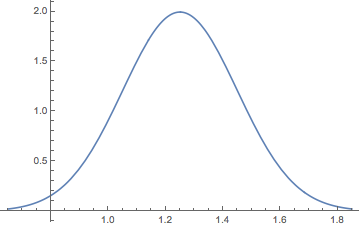
\includegraphics[width=0.8\textwidth]{fig3-1.png}
    \caption{Función de probabilidad normal, horas contra probabilidad}
    \label{fig:prob_dist1}
\end{figure}

Si se quiere saber la probabilidad de que un viaje en un bus cuya ruta se comporte de acuerdo a la descripción, se quiere saber $\mathbb{P}(X > 1.5)$. Lo cual, por propiedades básicas de la teoría de la probabilidad es igual a $1 - \mathbb{P}(X < 1.5)$ para variables aleatorias continuas. Para hallar esto, se estandariza la variable aleatoria $X$, de tal forma:

$$X \sim \mathcal{N} (\mu , \sigma ^2) \Rightarrow Z \sim \mathcal{N} (0,  1)$$
$$1 - \mathbb{P}(X < 1.5) = 1 - \mathbb{P}\left(Z < \frac{1.5 - \mu}{\sigma}\right) = 1 - \mathbb{P}\left(Z < \frac{1.5 - 1.25}{0.2}\right)$$
$$1 - \mathbb{P}(X < 1.5) = 1 - \mathbb{P}\left(Z < 1.25 \right) = 1 - 0.8944 = 0.10565$$

\pagebreak
La probabilidad que se halló, estaba acumulada en:

\begin{figure}[h]
    \centering
    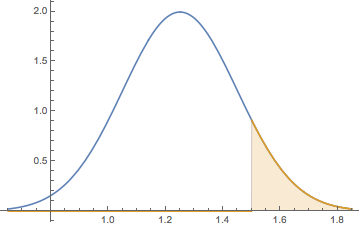
\includegraphics[width=0.8\textwidth]{fig3-2.png}
    \caption{Función de probabilidad normal, horas contra probabilidad.}
    \label{fig:prob_dist2}
\end{figure}

\item Bibiana va tarde a su trabajo y le indicará a su jefe el tiempo máximo que se
tardará en llegar a la oficina. Ella quiere indicarle un tiempo que, con una probabilidad de 0.9,
no exceda el tiempo de recorrido del SITP que acaba de abordar.

Se quiere hallar un $a$ tal que $\mathbb{P}(X < a) = 0.9$. Esto satisface la definición para que con ésta pobabilidad, el tiempo de demora de Bibiana no exceda $a$. Se estandariza este valor:

$$\mathbb{P}\left(Z < \frac{a - \mu}{\sigma} \right) = \mathbb{P}\left(Z < \frac{a - 1.25}{0.2} \right)  = 0.9$$

El valor para cual la variable aleatoria $Z \sim \mathcal{N} (0, 1)$, toma un valor tal que la probabilidad acumulda hasta tal valor sea $0.9$ es, según la tabla de probabilidad acumulada de la Normal estándar es $z = 1.29$. Luego:

$$\frac{a - 1.25}{0.2} = 1.29 \Rightarrow a = (1.29)(0.2) + 1.25 \Rightarrow a = 1.508$$

El tiempo que debe indicar Bibiana es de $1.508$ horas.

\pagebreak
\item Calcule la probabilidad de que un bus seleccionado al azar tenga un tiempo de
trayecto de exactamente una hora.\\

Dado que es una variable aleatoria continua, es imposible calcular la probabilidad puntual de un punto exacto del rango de la distribución, conceptualmente, y analíticamente, este tiende a cero.

$$\mathbb{P}\left(X = 1\right) = 0$$

\item ¿Cuál es la probabilidad de que en un trayecto seleccionado al azar haya tenido
un tiempo de recorrido entre 45 minutos y 1 hora?\\

Se pregunta por la probabilidad de que el timepo transcurrido en un viaje de un bus de la muestra cuyo recorrido se modela haciendo uso de $X$ esté entre 45 minutos y 1 hora exactamente. Es decir:

$$\mathbb{P}(45_{min} < X < 1_{hor}) = \mathbb{P}(0.75_{hor} < X < 1_{hor})$$
 
Por propiedades básicas de las distribuciones de probabilidad:
 
$$\mathbb{P}(0.75_{hor} < X < 1_{hor}) = \mathbb{P}(X < 1_{hor}) - \mathbb{P}(X < 0.75_{hor})$$

Estandarizando la variable $Z \sim \mathcal{N} (0, 1)$, se tiene:

\begin{equation}
    \begin{aligned}
    \mathbb{P}\left(Z < \frac{1 - \mu}{\sigma} \right) - \mathbb{P}\left(Z < \frac{0.75 - \mu}{\sigma} \right) =
    \\
    \\
     \mathbb{P}\left(Z < \frac{1 - 1.25}{0.2} \right) - \mathbb{P}\left(Z < \frac{0.75 - 1.25}{0.2} \right) = 
     \\
     \\
     \mathbb{P}\left(Z < -1.25 \right) - \mathbb{P}\left(Z < -2.5 \right) =
     \\
     \\
     \left[ 1 -  \mathbb{P}\left(Z < 1.25 \right) \right] - \left[ 1 - \mathbb{P}\left(Z < 2.5 \right) \right] = 
     \\
     \\
      -\mathbb{P}\left(Z < 1.25 \right) +  \mathbb{P}\left(Z < 2.5 \right) =
      -0.8944 + 0.9928 
      \\
      = 0.0994401
\end{aligned}
\end{equation}

\pagebreak
La probabilidad que se halló, estaba acumulada en:

\begin{figure}[h]
    \centering
    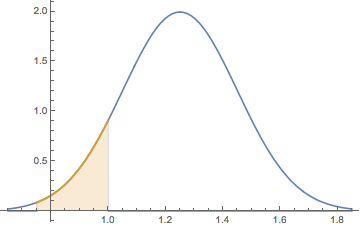
\includegraphics[width=0.8\textwidth]{fig3-3.png}
    \caption{Gráfica de probabilidad de que se llege con un timepo entre 45 minutos y 1 hora.}
    \label{fig:prob_dist2}
\end{figure} 

\item Calcule el valor de la constante $c$ que garantiza que, con probabilidad de 0.90, el
tiempo de recorrido de un bus seleccionado al azar estará intervalo $\left[ 1.25 - c,\ 1.25 + c\right]$.\\

El valor pedido, es un $c$ tal que para algún $X$, la probabilidad de que esté entre $1.25 - c$ y $1.25 + c$ sea $0.90$. Por principios básicos de probabilidad y de distribuciones de probabilidad:

\begin{equation}
    \begin{aligned}
   \mathbb{P}\left(1.25 - c < X < 1.25 + c \right) = 0.9 \Rightarrow   \\
  \mathbb{P}\left(X < 1.25 + c\right) -   \mathbb{P}\left(X < 1.25 - c\right) = 0.9 \Rightarrow\\
  \mbox{Al estandarizar se obtiene:} \\
  \mathbb{P}\left(Z < \frac{1.25 + c - \mu}{\sigma} \right) - \mathbb{P}\left(Z < \frac{1.25 - c - \mu}{\sigma} \right) = 0.9 \Rightarrow \\
  \mathbb{P}\left(Z < \frac{1.25 + c - 1.25}{0.2} \right) - \mathbb{P}\left(Z < \frac{1.25 - c - 1.25}{0.2} \right) = 0.9 \Rightarrow  \\
  \mathbb{P}\left(Z < \frac{c}{0.2} \right) - \mathbb{P}\left(Z < \frac{- c}{0.2} \right) = 0.9 \\
\end{aligned}
\end{equation}

\pagebreak
Por propiedades de las distribuciones normales

$$  \mathbb{P}\left(Z < \frac{c}{0.2} \right) - \left[ 1 - \mathbb{P}\left(Z < \frac{c}{0.2} \right) = 0.9 \right] $$
$$  \mathbb{P}\left(Z < \frac{c}{0.2} \right) - 1 + \mathbb{P}\left(Z < \frac{c}{0.2} \right) = 0.9 $$
$$  2\left(\mathbb{P}\left(Z < \frac{c}{0.2} \right)\right) - 1  = 0.9 \Rightarrow \mathbb{P}\left(Z < \frac{c}{0.2} \right) = \frac{1.9}{2} = 0.95$$

Según la tabla de distribución normal estándar, el primer valor $z$ para el cual $\mathbb{P}\left(Z < z \right) = 0.9$ es $1.65$. Luego, $\frac{c}{2} = 1.65 \Rightarrow c = 0.33$.



\end{enumerate}

\pagebreak
\section{Función Generatriz de Momentos}

\begin{enumerate}[(a)]

\item ¿Cuál es el número esperado de fallas en las máquinas durante un mes?\\

Como $\Psi_{X}(t) = e^{6 \times \left( e ^{t} - 1 \right)}$ es la función generatriz de momentos para la variable aleatoria que representa el número de fallas mensuales que tiene la máquina, y por la teoría se sabe que $\Psi_{X}^r(t = 0) = \mathbb{E}(X^r)$; entonces el primer momento central equivale a $\mathbb{E}(X^1) = \mathbb{E}(X)$.

$$\Psi'_{X}(t) = 6 \times e ^{6 \times (-1 + e^t) + t}$$
$$\Psi'_{X}(0) = 6 \times e ^{6 \times (-1 + e^0) + 0} = 6 \times e ^{6 \times (-1 + 1)} = 6 \times e ^{0} = 1$$

\item ¿Cuál es la varianza del número de fallas en las máquinas durante un mes?\\

Como $\Psi_{X}(t) = e^{6 \times \left( e ^{t} - 1 \right)}$ es la función generatriz de momentos para la variable aleatoria que representa el número de fallas mensuales que tiene la máquina, y por la teoría se sabe que $\Psi_{X}^r(t = 0) = \mathbb{E}(X^r)$; entonces el segundo momento central equivale a $\mathbb{E}(X^2)$.

$$\Psi'_{X}(t) = 6 \times e ^{6 \times (-1 + e^t) + t}$$
$$\Psi''_{X}(t) = 6 \times e^{6 \times \left(e^t-1\right)+t} \times \left(6 \times e^t+1\right)$$
$$\Psi''_{X}(0) = 6 \times e^{6 \times \left(e^0-1\right)+0} \times \left(6 \times e^0+1\right) = 6 \times e^{6 \times \left(1-1\right)+0} \times \left(6 \times 1+1\right)$$
$$\Psi''_{X}(0) = 6 \times e^{0} \times 7 = 6 \times 7 = 42 = \mathbb{E}(X^2)$$
\begin{center}
	\line(1,0){300}
\end{center}
$$\mathbb{V}(X) = \mathbb{E}[X^2] - \mathbb{E}[X]^2 = \Psi''_{X}(0) - (\Psi'_{X}(0))^2 $$
$$\mathbb{V}(X) = 42 - 6^" = 42 - 36 = 6 $$

\item Halle su función generatriz de momentos. Muestre todo el procedimiento.\\

Sea $f_{Y}(y) : \mathbb{R} \mapsto \mathbb{R}$, una función definida por la expresión $f_{Y}(y) = 1/20 \iff y \in (1, 20) \subset \mathbb{R} \wedge f_{Y}(y) = 0 \iff y \notin (1, 20) \subset \mathbb{R}$. Sea $g(t) = e^{t \times y}$, definida sobre $\mathbb{R}$ para todo intervalo de definición de la variable $y$. El producto funcional de ambas funciones, se define através de la variable $y$, por lo que las porciones donde $y$ valfa cero sobre algun intervalo de por lo menos una de las funciones, entonces en el mismo intervalo, el producto funcional es cero. Acontinuación se ilustra el producto funcional de las funciones definidas en este párrafo sobre un intervalo de interés.

\[ f_{Y}(y) = \begin{cases} 
      \frac{1}{20} & 0 < x < 20 \\
      0 & d.l.c
   \end{cases}
\]

$$g(t) = e^{t \times y}$$

\begin{figure}[h]
    \centering
    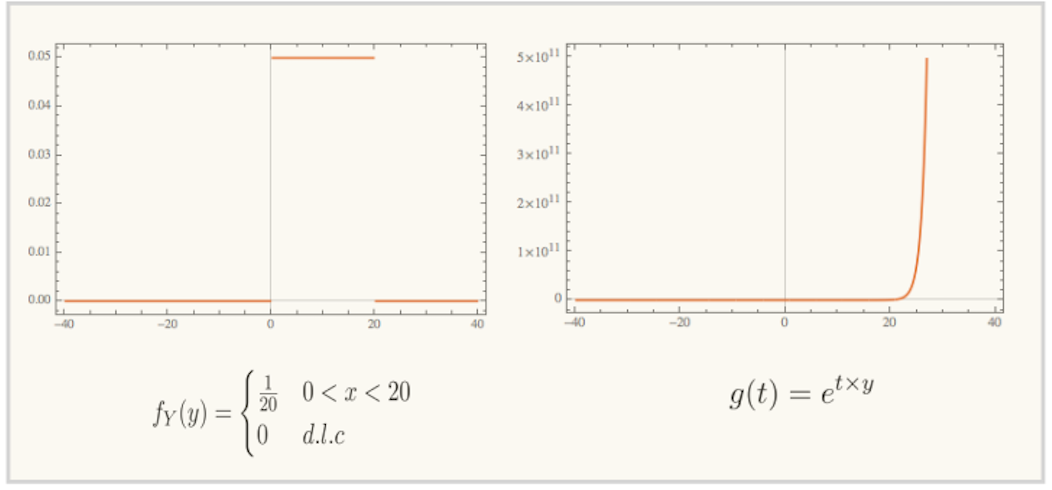
\includegraphics[width=1\textwidth]{fig4-1.png}
    \caption{Función de distribución de probabilidad y función para la generación de momentos centrales de una distribución.}
    \label{fig:prob_dist2}
\end{figure}

$$\Psi_{Y}(t) = \int_{- \infty}^{\infty} \left( e^{y \times t} \times f_{Y}(y)\right)\ dy = \int_{\mathbb{R}[Y]} \left( e^{y \times t} \times f_{Y}(y)\right)\ dy$$
$$\Psi_{Y}(t) = \int_{0}^{20} \left( e^{y \times t} \times f_{Y}(y)\right)\ dy = \int_{0}^{20} \left( e^{y \times t} \times \frac{1}{20}\right)\ dy$$
$$\Psi_{Y}(t) = \frac{1}{20} \int_{0}^{20} e^{y \times t}\ dy = \frac{1}{20} \left[\left.   \frac{e^{t \times y}}{t} \right|_{y=0}^{y = 20}
 \right] = \frac{1}{20} \left[\frac{e^{20 \times t}}{t} -  \frac{e^{0 \times t}}{t} \right]$$
$$\Psi_{Y}(t) = \frac{1}{20} \left[\frac{e^{20 \times t} - e^{0 \times t}}{t} \right] = \frac{1}{20} \left[\frac{e^{20t} - 1}{t} \right] = \frac{e^{20t} - 1}{20t} $$

\end{enumerate}

\end{document}